% omci.tex:

\chapter{OPTICAL MAMMOGRAPHY CO-IMAGER (OMCI)} % all caps please
\label{chap:omci}
\ac{OMCI} is a high-density breast multi-subsystem devide designed to be used in conjunction with existing x-ray mammography systems or as a standalone system for \ac{DOT}. It integrates four subsystems: a mechanical breast compression stage to resemble clinical mammography, a frequency-domain subsystem for recovering absolute tissue optical properties, a wide-field transmission-based diffuse optical subsystem, and high-resolution breast surface acquisition system. Although \ac{OMCI} is composed of four separate subsystems working in tandem, in this chapter, we will briefly provide an overall instrument description but will focus on design and characterization of the dual-camera structured light imaging (\ac{SLI}) breast shape acquisition system used for improving diffuse optical tomography image reconstructions.


\section{Introduction} %significance
\label{chap:omci:introduction}
Breast cancer is the most commonly diagnosed cancer in women worldwide with an estimated 1,918,030 new cases in 2022 in the United States alone~\cite{Siegel2022}. Screening and diagnostics of breast cancer is done through structural or functional breast imaging using multiple breast imaging modalities. X-ray mammography and \ac{DBT}) are the primary breast cancer screening techniques~\cite{Secretan2015} used for early detection to reduce mortality rates~\cite{Tabar2003}. Modalities such as magnetic resonance imaging (\ac{MRI}) and positron emission tomography (\ac{PET}) are used less frequently than x-ray due to their high cost and use of radioactive isotopes~\cite{Secretan2015}. Despite its recommendation for screening, not only does x-ray mammography expose patients to ionizing radiation but it also suffers from a high false-positive diagnostic rate~\cite{Tabar2003, Elmore1998}. The modality lacks both strong structural contrast between healthy and tumor tissue, and the ability to quantify tissue functions to assess benign versus malignancy~\cite{Leff2008}. These limitations have led researchers to investigate using \ac{DOT}) techniques to characterize the breast tumor's physiology to lower false-positive diagnoses. 

Unlike x-ray mammography, \ac{DOT} is an imaging modality that uses non-ionizing \ac{NIR} radiation to yield three-dimensional (3-D) maps of the optical properties of illuminated tissue~\cite{Boas2001, Dehghani2009, Yamada2014, Hoshi2016}. Biological tissues' primary absorbers in the spectral window from around 600 to 1000~nm have relatively low absorption, allowing \ac{NIR} light to penetrate through centimeters of tissues~\cite{Gibson2005}. This allows the quantification of physiological properties such as hemoglobin concentration, blood volume, and blood oxygen saturation~\cite{Leff2008, Boas2001}. Malignant tumors generally demand a greater blood supply than their surrounding tissues, leading to increased light absorption that can be delineated using spectroscopy and imaging methods, making \ac{DOT} particularly useful for breast cancer imaging diagnosis~\cite{Wang2022, Vavadi2014, Flexman2013, Choe2009, Taroni2005}. Unfortunately, \ac{DOT} images are known for low spatial resolution largely caused by the high scattering properties of biological tissues~\cite{Boas2001}. 

The low spatial resolution of \ac{DOT}~\cite{Li2010} can be improved by a multi-modal approach with x-ray mammography~\cite{Zimmermann2017, Deng2015, Deng2015a, Fang2009a}. The high scattering present in the breast tissue redirects photons to traverse large overlapping probing volumes before their detection, greatly reducing the locality of the measurements and resulting in blurry images. Mathematically, this is reflected as the severe ill-posedness of the inverse problem. Parallel-plate compression of breast tissues has been used in an x-ray mammography scan to minimize overlapping tissues and has also been explored for a number of standalone~\cite{Choe2009, Culver2003} and multi-modal \ac{DOT} breast imaging systems~\cite{ZhuReview2020, Fang2009a, Krishnaswamy2012}. Multi-modal imaging approaches have been developed by leveraging tissue structural priors obtained from high-resolution imaging methods such as magnetic resonance imaging~\cite{Ghussein2013,Ntziachristos2002} and ultrasound~\cite{Zhu2010}. These approach leverage the advantages of multiple modalities---they leverage high quality structural images to constrain the \ac{DOT} inverse problem for more accurate tissue physiology reconstructions. 

Additionally, the \ac{DOT} reconstruction can also be improved by constraining the inverse problem through more accurate surface representations of the breast. Obtaining breast surface information to aid quantitative analysis of imaging data has garnered interest from a number of applications, including \ac{DBT}~\cite{Rodriguez2017} and \ac{MRI} scans~\cite{Pallone2014, Ortiz2012}. For multi-modal \ac{DOT} systems, the 3-D shape of the breast can be estimated using the structural imaging modality such as \ac{DBT}~\cite{Fang2011} or \ac{MRI}~\cite{Brooksby2006}. When a 3-D imaging modality is not available, two-dimensional (2-D) mammography~\cite{Deng2015a} has also been used to provide the shape information. In such case, a simple way to recover a 3-D breast surface is to extrude the 2-D breast contour along the compression axis~\cite{Kruger2013, Kalbhen1999}, or sweep the 2-D breast contour along the contour line extracted from an orthogonal view~\cite{Kita1998}. These methods either rely on assumptions about the 3-D location of certain features (e.g. mamilla position) or assume a constant curvature of the breast along the sweeping direction. For more accurate reconstructions of tissue optical properties, especially near the surface, measuring 3-D breast surface accurately can be greatly beneficial.

Accurately acquiring breast 3-D surface shapes has gained clinical acceptance due in large part to the plastic and reconstructive surgery communities~\cite{Chang2015, Losken2005}. The two prominent techniques for 3-D breast surface imaging are stereophotogrammetry and laser scanning~\cite{Yang2015}. Stereophotogrammetry works by overlaying multiple images of an object taken from different view angles and triangulating the location of the object based on matching features in the multiple images~\cite{Ju2016, Galdino2002, FangOSA2012}. In addition to requiring multiple cameras to increase accuracy~\cite{Henseler2012}, this technique is also heavily influenced by lighting conditions since features need to be extracted from multiple viewpoints~\cite{Henseler2011}. Another limitation is the ``ptosis error'' seen during scanning of ptotic or larger breasts~\cite{Nahabedian2003}. This arises due to the small field of view of stereophotogrammetry systems, leading to inaccuracies in breast surface and volume estimations due to the portions of the breast that are not illuminated. Laser scanning is a surface imaging technique in which rays from a laser beam are reflected off an object and detected by a detector~\cite{Kovacs2006}. Although laser-based acquisition systems can produce more accurate surfaces~\cite{Kovacs2006b}, these systems tend to be expensive~\cite{Kovacs2007, Koch2011} and require the need for very precise setups~\cite{Thomson2009}. Recently, the use of patterned-lasers and orientation-sensitive detectors has led to an increase in portable 3-D laser scanning devices~\cite{Kuzminsky2012}. While low-cost laser-based depth sensors have been widely deployed in game consoles such as Xbox or PlayStation, they are only designed to achieve relatively low spatial accuracy compared to dedicated 3-D scanners. Still, patterned-laser-based surface acquisition systems generally require a minimum scanner-to-target distance of 35~cm~\cite{Ametek2002, Artec3D2022}. Additionally, their typical housing is too large to fit between mammography compression plates~\cite{Artec3D2022, Pallone2014}. Bulky instrumentation and long minimum working distance requirements make stereophotogrammetry and laser scanning techniques infeasible in the confined, low-light mammography setting. 

Another widely used 3-D surface acquisition technique is \ac{SLI}~\cite{Yang2020, Zhang2018}. \ac{SLI} works by illuminating an object with two-dimensional spatially varying patterns with a projector and capturing images from the illuminated object using cameras~\cite{Geng2011}. The distortion of the specially designed patterns provides information regarding the shape of the object. Calibration of the camera-projector system is easily done by capturing images of a known planar pattern (e.g. a checkerboard). With the ability to use off-the-shelf components, a simple setup with a single projector and camera, and a robust and simple calibration method, \ac{SLI} is positioned to provide accurate, fast, and cost-effective breast surface scanning~\cite{Yang2020}. However, similar to most patterned-laser surface scanners, commercially available \ac{SLI} systems have long minimal working distance requirements and large assemblies that cannot readily fit within the confined mammography compression plates~\cite{Zhang2018, Rodriguez2017}.

Our approach to lowering false-positive diagnoses is two-fold. We first aim to improve \ac{DOT} reconstruction through more accurate surface representations of the compressed breast. Second, we aim to develop a standalone \ac{DOT} breast imaging system that leverages structural information through the registration of the \ac{DOT} reconstruction with prior x-ray mammographies. Our group has primarily focused on the latter through the development of both multi-modal \ac{DOT} reconstruction algorithms~\cite{Deng2015} and multi-modal (\ac{DOT} and \ac{DBT}) instrumentation that can work independently~\cite{Carp2006,Carp2008,Carp2013} or in conjunction with existing mammography systems~\cite{Fang2009,Zimmermann2017}. The approach to build \ac{DOT} systems that can work independently and integrate with existing mammography systems is commercially intriguing, since it can lower acquisition costs and maximize previous investments made into clinical instrumentation. We will take this same approach in our first aim---that is, the \ac{SLI} surface acquisition system we build will also have the capability to function independently or be easily integrated into existing mammography systems. 

In this chapter, we first describe the overall \ac{OMCI} instrument and its subsystems. We then describe the design of the \ac{SLI} breast scanner and detail the methods for adaptive illumination for subject-specific skin tones as well as approaches to reduce specular reflection from the compression plates. Next, we compare several traditional surface acquisition methods that leverage mammography images against our \ac{SLI}-based breast surface acquisition system and quantify the impact of improved breast surface acquisition on the recovery of breast lesions using a series of simulations. Finally, we demonstrate \ac{OMCI}'s use on healthy volunteers.



\section{Methods}
\label{chap:omci:methods}

%%% Subsection %%%
\subsection{OMCI Instrument}
\begin{figure}
    \begin{center}
    \subfigure[]{\label{fig:OMCISystemA}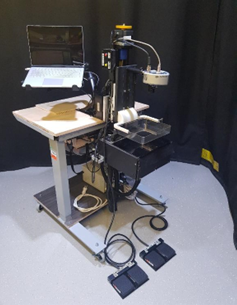
\includegraphics[width=.4\textwidth]{fig/omci/OMCISystemImage_1.png}}
    %\subfigure[]{\label{fig:OMCISystemB}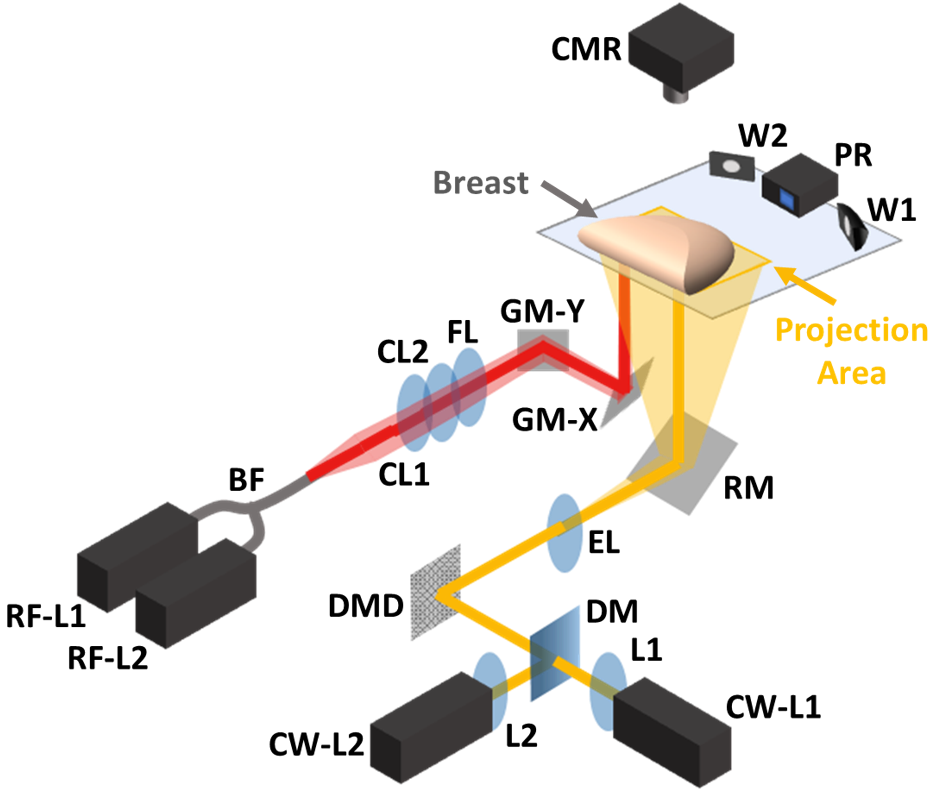
\includegraphics[width=.5\textwidth]{fig/omci/OMCISystemSketch.png}}
    \end{center}
    \caption{The \ac{OMCI} system in its fully compressed state. } 
    \label{fig:OMCISystem}
\end{figure} 

%\subsubsection{Mechanical stage and auxiliary sensors suite}
\ac{OMCI} is composed of a linear stage mounted on a vertical rotary stage. The breast is compressed by a pair of acrylic plates, with one plate mounted at the stationary end of a linear stage (MN10-0160-M02-31 BiSlide, Velmex, NY, USA). Under the bottom compression plate is a box that encloses many of the optical components of \ac{OMCI}. An acrylic mammography compression plate is mounted on the moving gantry of the linear stage, allowing for a plate separation ranging from 300~mm (fully released) to 0~mm (fully closed). A linear encoder (ETI Systems, Carlsbad, CA, USA) is connected between the pair of compression plates to measure their separation. The entire breast compression assembly is mounted on a rotatory table (306045-1-s-M04-C376, Lintech, Monrovia, CA, USA), controlled by a foot pedal to permit mammography-like lateral-oblique compression. A motor driver interface (VXM-2, Velmex Inc., USA) allows both stages to be actuated independenly by their stepper motor (NEMA 34 PK296 Stepper Motor, Oriental Motor Corporation, MA, USA). Two limit switches (BiSlide Push Button, Velmex Inc., NY, USA) confine the translation stage range. A reed switch (L06 Non-Contact Reed Switch, LinTech Motors, CA, USA) is used for homing the rotary stage. Four load sensors (SEN-10245, SparkFun, CO, USA) hold up the bottom compression plate and measure the pressure applied on the breast.  This design specifically enables registration of structural information from separately acquired mammography scans with the \ac{DOT} images using the methods detailed in our previous studies~\cite{Deng2015}.

%\subsubsection{Galvo-based frequency-domain subsystem}
%\label{sec:RF}
While the breast is in compression, it is illuminated with an \ac{FD} and a \ac{WF} subsystem. Bulk tissue properties are determined using a \ac{FD} subsystem~\cite{Zimmermann2016} that utilizes two laser modules (HL6750MG and HL8338MG, Thorlabs GmbH, Germany) coupled to bifurcated fiber bundle (BFY400LS02, Thorlabs GmbH, Germany). The frequency multiplexed light is driven into the \ac{OMCI} box where a dual-axis galvo motor (GVS002, Thorlabs GmbH, Germany) redirects it onto different positions on the bottom of the compressed breast. A fixed detector on the top compression plate directs the light to a frequency-domain detector (C5331-04, Hamamatsu, Japan) for collection. The \ac{WF} subsystem illuminates the breast from below using a \ac{CW} projector (P300 Neo, Aaxa Technologies, USA) while a \ac{EMCCD} camera (Andor Luca R, Oxford Instruments, U.K) located above the compression plate samples the dual-wavelength light transmitted through the breast. Both the \ac{FD} and \ac{WF} subsystems are controlled through the \ac{OMCI} \ac{GUI} written in MATLAB. 


%%% Subsection %%%
\subsection{Dual-camera SLI breast surface scanning system}
\label{sec:sli}
\begin{figure}
	\begin{center}
	\subfigure[]{\label{fig:mammography_top}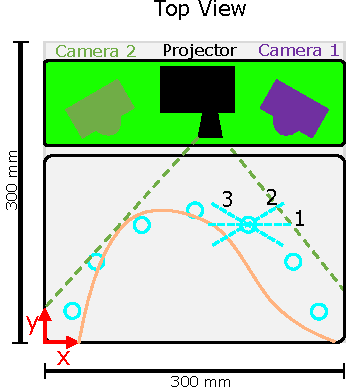
\includegraphics[height=5cm]{fig/omci/mammography_top.pdf}}
	\subfigure[]{\label{fig:mammography_side}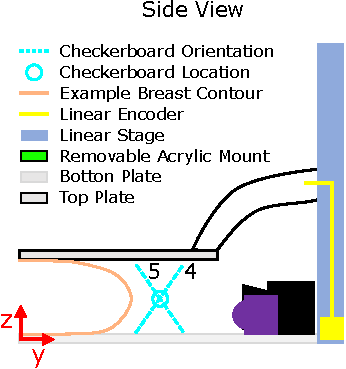
\includegraphics[height=5cm]{fig/omci/mammography_side.pdf}}
	\subfigure[]{\label{fig:mammography_setup}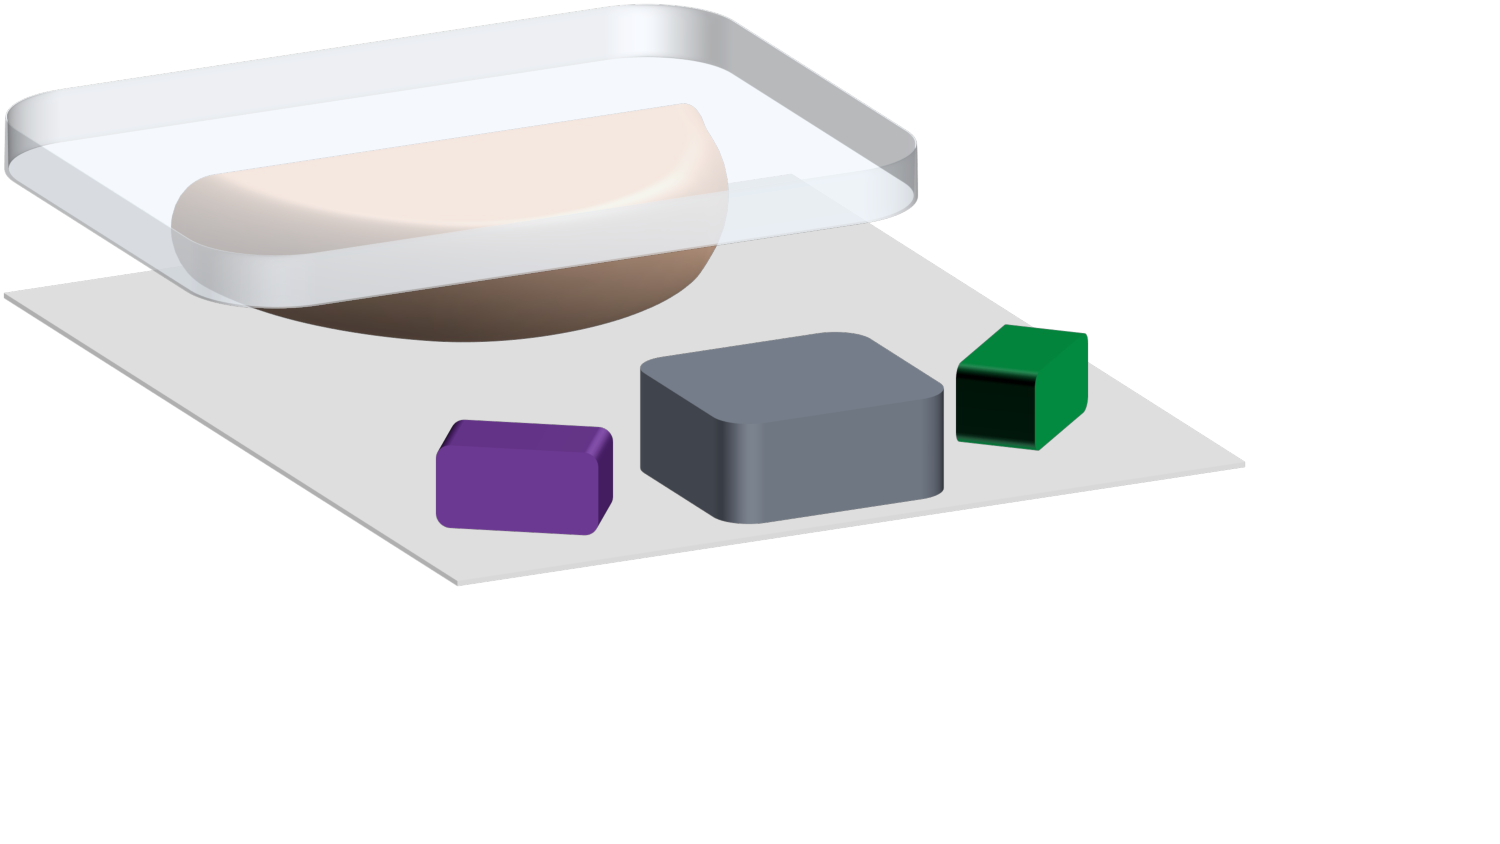
\includegraphics[width=5cm]{fig/omci/sli_model.pdf}}
	\end{center}
	\caption{ (a) Top-view of the breast compression compartment -- upper: \ac{SLI} system; bottom: horizontal cross-section (orange line) of the compressed breast with blue circles indicating the placement of the checkerboard used for system calibration. Numbers 1-5 indicate the 5 board orientations repeated at each location for calibration. (b) Side-view of the breast compression plates, showing the linear translation stage (blue bar on the right) and a linear encoder (in yellow), and  (c) 3-D rendering of the \ac{SLI} system, an acrylic bottom plate and an acrylic compression plate (top). } 
	\label{fig:mammographysetup}
\end{figure} 

The \ac{SLI} system is embedded between the compression plate to provide accurate measurement of the breast surface [Fig.~\ref{fig:mammography_setup}]. This low-profile \ac{SLI} scanner has a dimension of 30$\times$10$\times$4.8~cm$^3$ and is attached to the stationary compression plate, on the side facing the patient's breast [Fig.~\ref{fig:sli_setup}]. It consists of a central projector (P2-B DLP Pico Projector, AAXA Technologies, Irvine, CA, USA) and two USB cameras (C525, Logitech, Lausanne, Switzerland) to reconstruct a 3-D surface of the compressed breast. The \ac{SLI} scanner is designed to have a relatively short scanner-to-target distance, typically less than 15~cm, and a vertical profile of less than 3~cm to permit scanning breasts with a wide range of sizes. A laptop is used to control the data acquisition, including illumination pattern generation, projection, camera image acquisition, and translation stage control via an interface written in MATLAB (R2017b, Mathworks, Natick, MA, USA).

Gray-code-based binary patterns~\cite{Inokuchi1984} are sequentially illuminated onto the breast surface and captured using both USB cameras. These patterns are characterized by their pattern order, $P$. A pattern set of $P=3$ results in 3 sequences which are a reflected binary of the previous (``01'', ``0110'', and ``01100110''). Four bar patterns are created for each sequence (a horizontal black and white bar pattern, a vertical black and white bar pattern, and the complimentary pattern of each)~\cite{Sels2019}. The digits correspond to the white (``1'') and black (``0'') bars. In addition, a full-bright (white) and full-dark (black) pattern are added to each pattern set. Thus, a pattern set of $P=3$ results in $4\times P+2$ illumination bar patterns. Complimentary Gray-code-based illumination pattern sets are used due to their robustness to decoding errors~\cite{Moreno2012}. The two USB cameras have overlapping field-of-views and sequentially capture images of the breast during each illumination pattern at an exposure time of 250~ms. Dual-camera simultaneous acquisition allows the \ac{SLI} system to capture the curved surface of breasts of varied sizes without moving components. 

\subsubsection{Special data acquisition considerations}\label{sec:special}
% skin tone
Skin tone differences are known to affect light-based surface reconstruction accuracy, especially in low-light settings. To account for skin tone variations, the normalized illumination patterns are multiplied by a scaling factor $\alpha$ ranging from 0 to 1 to prevent camera saturation. The scaling factor for a camera is calculated prior to data acquisition by first illuminating a full-bright pattern with $\alpha=1$ onto the breast and capturing a single image using the camera. If the maximum pixel value of the captured image is above a preset threshold, $\alpha$ is decreased and the breast is re-illuminated with a full-bright pattern multiplied by the new $\alpha$ value. This procedure is repeated until the maximum pixel value of the captured image is less than 95\% of the camera's maximum allowable pixel value. This entire procedure takes an estimated 8 seconds to complete and is repeated for each camera.

\begin{figure}
	\begin{center}
	\subfigure[]{\label{fig:sli_setup}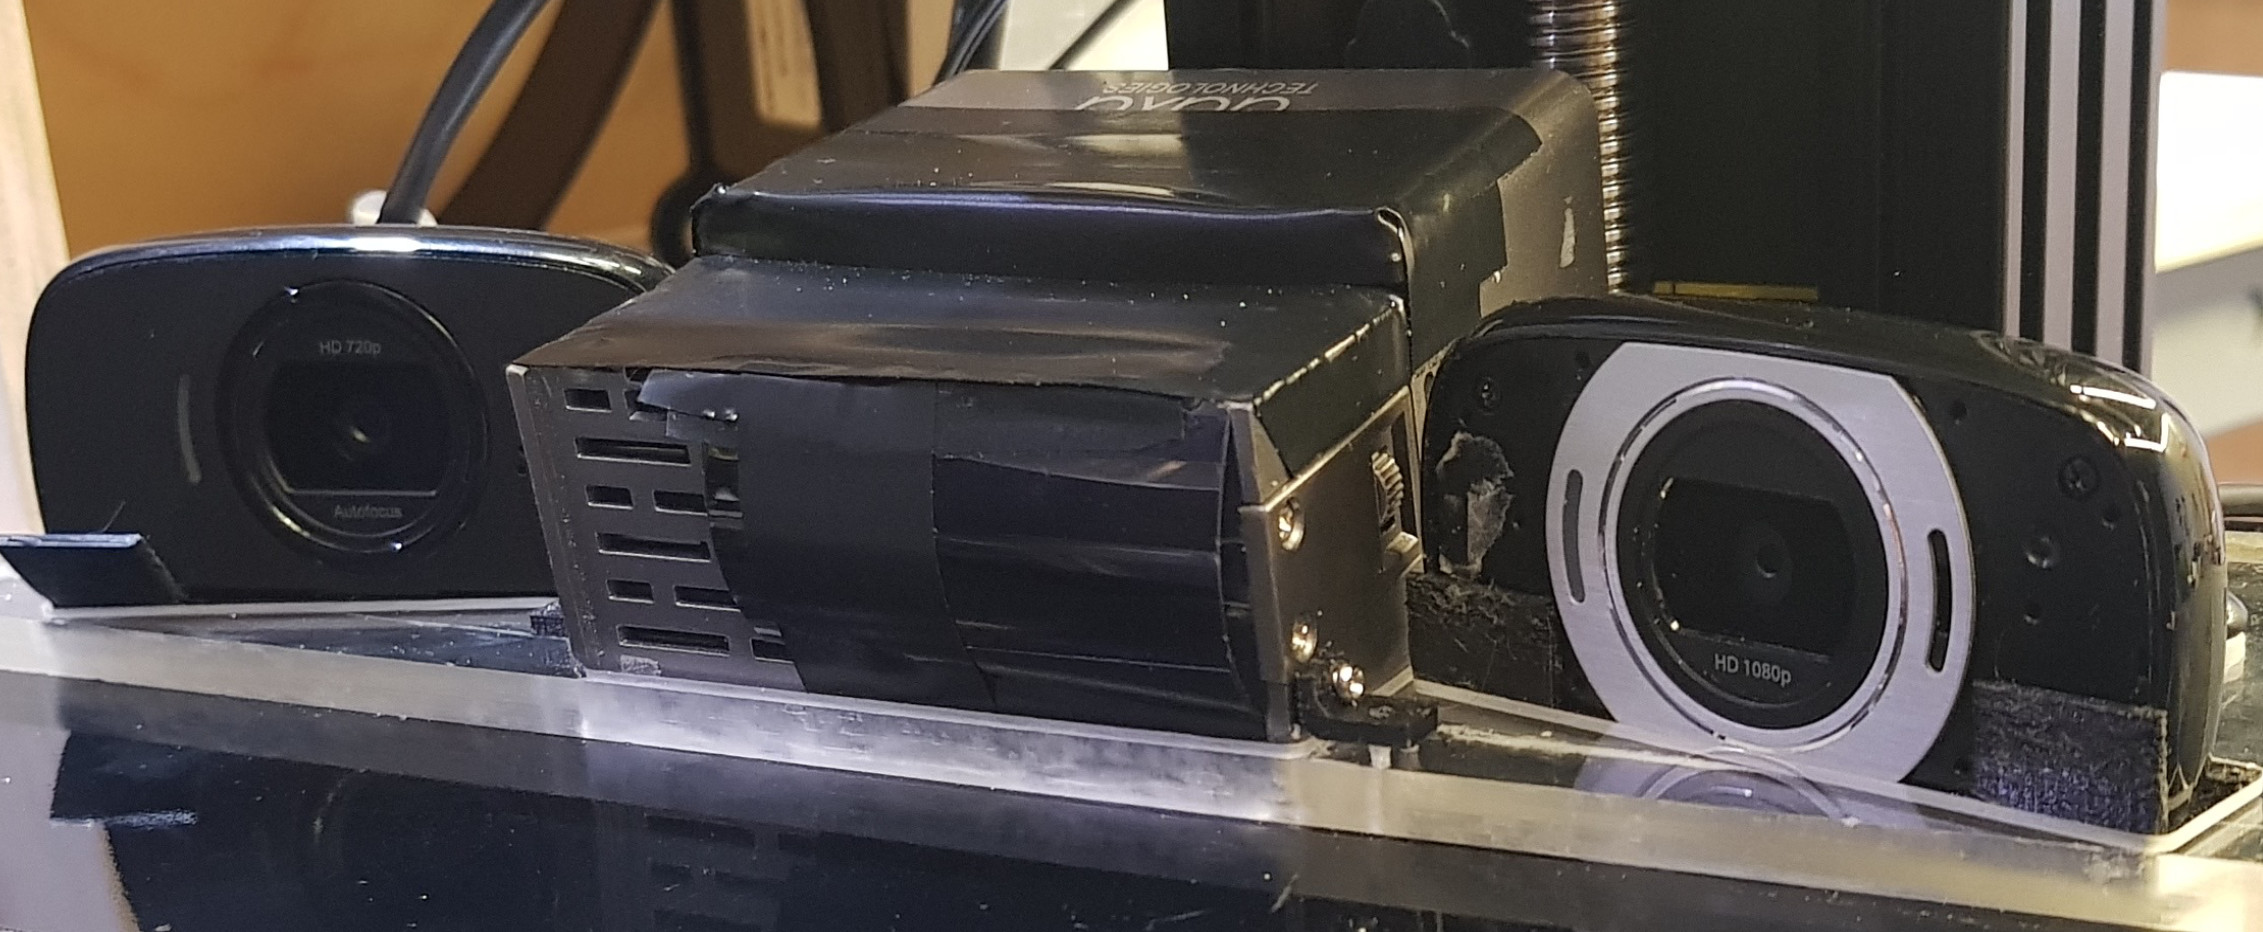
\includegraphics[height=2.4cm]{fig/omci/sli_photo.jpg}}
	\subfigure[]{\label{fig:artifact1}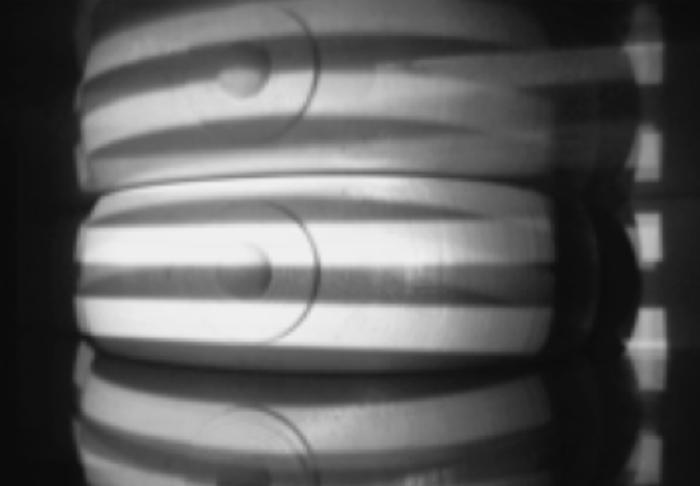
\includegraphics[height=2.4cm]{fig/omci/bars_artifact.png}}
	\subfigure[]{\label{fig:artifact2}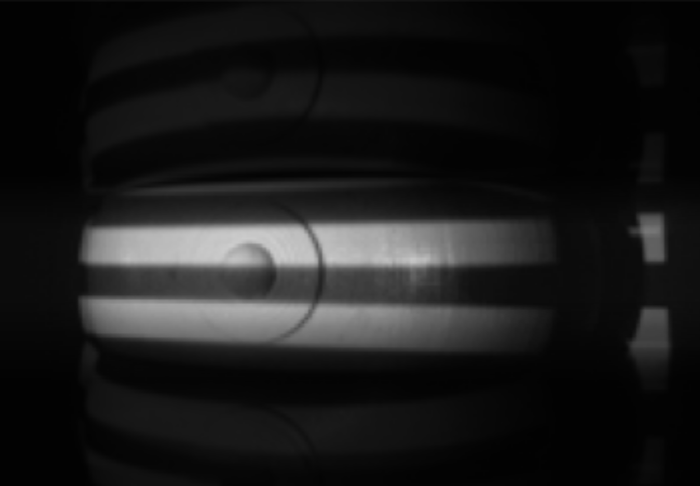
\includegraphics[height=2.4cm]{fig/omci/bars.png}}
	\end{center}
	\caption{(a) Front-view photo of the \ac{SLI} system. Cameras and projectors are embedded in an acrylic mount to prevent the need for re-calibration. (b) Horizontal bar patterns reflecting off the top compression plate and onto the breast show curved illumination bar artifacts when the scaling factor $\alpha$ is set to 1. In (c), we show the same illumination pattern with thickness-informed masking eliminating the curved bar artifacts by cropping the patterns exceeding the breast surface before projection. Additionally, the scaling factor is automatically calculated to prevent camera saturation.} 
	\label{fig:barartifacts}
\end{figure} 

% encoder-informed masking
Additionally, specular reflections from the acrylic compression plates, shown in Fig.~\ref{fig:artifact1}, can produce vertically mirrored breast surfaces. To minimize such specular reflection, we use dynamic pattern masking based on real-time separation readings provided by a linear encoder. By limiting the vertical span of the illumination patterns, the patterns are projected onto the compressed breast surface without generating strong direct specular reflections from the top and bottom compression plates, as shown in Fig.~\ref{fig:artifact2}.

\subsubsection{SLI system calibration and re-projection errors}
A standard \ac{SLI} camera-projector calibration is performed prior to image acquisition and is described in detail in~\cite{Moreno2012}. For each camera-projector pair, a checkerboard pattern is fully illuminated in multiple positions and the corner locations are estimated in the projector's default coordinate system using a robust pixel classification algorithm~\cite{Xu2007}. The camera and projector's intrinsic parameters (optical center and focal lengths) are estimated using a calibration method described in~\cite{Zhang2000} by fixing a world coordinate system to the calibration checkerboard plane. 

The projector's extrinsic parameters (rotation and translation from camera to projector) are calculated using a simple stereo camera calibration~\cite{Bouguet2004} that treats the projector as a secondary camera. This results in a rotation matrix and a translation vector relating the camera's coordinates to the projector's coordinates. Once the 3-D coordinates of all the corners of the checkerboard are computed using the camera's (and projector's) intrinsic and extrinsic parameters, the corners are ``reprojected'' onto all the images for which they appear. The re-projection error is defined as the average distance between the re-projected corner locations and the actual corner location. 

\subsubsection{SLI system acquisition}
The same acquisition procedures are used for both calibrating the system and acquiring breast shape measurements (Fig.~\ref{fig:sli_flowchart}). A single acquisition refers to the image capture of all illumination patterns by both cameras. Camera-projector calibration requires an acquisition at each checkerboard position. During breast measurements, the acquisition is preceded by the determination of the saturation scaling factor $\alpha$ and masking of the patterns. Patterns during calibration are not masked since the calibration is done with the system fully uncompressed. 

\begin{figure}
    \begin{center}
    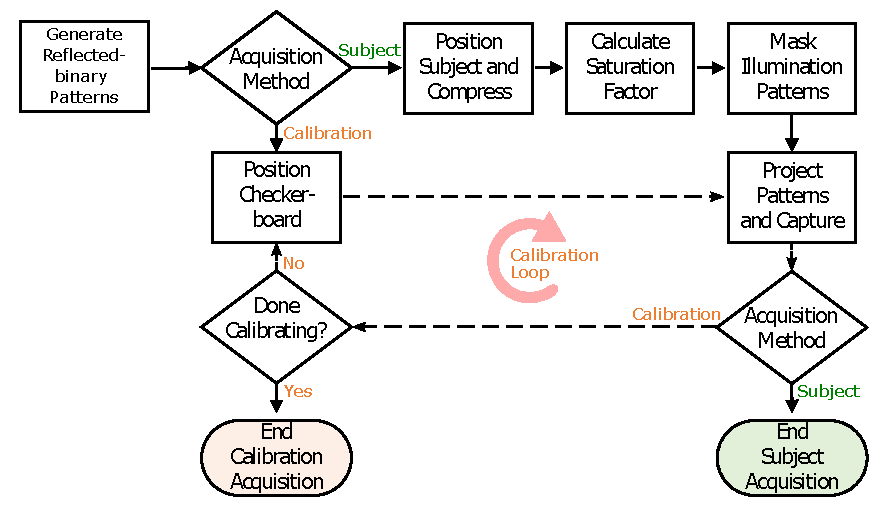
\includegraphics[width=.9\textwidth]{fig/omci/sli_flowchart.pdf}
    \end{center}
    \caption{Flow chart of image acquisition for both subject measurements and system calibration. Subject measurements calculate a saturation scaling factor and mask the illumination patterns prior to projecting patterns. System calibration measurements do not mask the illumination patterns and project at full intensity. The calibration loop (dashed lines) is repeated for each location and orientation of the calibration checkerboard.} 
    \label{fig:sli_flowchart}
\end{figure} 

%%% Subsection %%%
\subsection{Alternative breast surface reconstruction methods for assessing SLI surface accuracy}
To evaluate the accuracy of the \ac{SLI} system, we compare its output against alternative surface acquisition methods. Each method estimates the surface of a 3-D breast derived from a \ac{DBT} scan.

\begin{figure}
    \begin{center}
    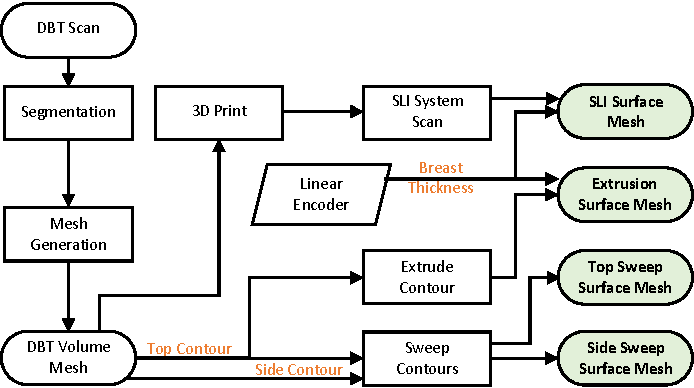
\includegraphics[width=.9\textwidth]{fig/omci/mesh_flowchart2.pdf}
    \end{center}
    \caption{Generation of breast surface meshes using multiple acquisition methods. The \ac{DBT} volumetric mesh is created from segmented scans. The extrusion surface mesh is created by extruding the top contour to the breast thickness. The top and side contours of the \ac{DBT} mesh are swept to create top and side surface meshes. The \ac{SLI} mesh is created by scanning a 3-D printed breast phantom and trimming the resulting point-cloud using the linear encoder measurements. The surface estimation error is calculated for each of the surface meshes by comparing the surface estimations to the \ac{DBT} mesh. All surface meshes are converted to volumetric meshes for validating the effect of surface estimation methods on inclusion reconstruction.}
    \label{fig:mesh_flowchart}
\end{figure} 

\subsubsection{Reference breast phantom fabrication}
Fig.~\ref{fig:mesh_flowchart} shows the process of creating surface meshes from \ac{DBT} scans. Scans were obtained from radiology data from \ac{TCGA} breast Invasive Carcinoma collection~\cite{Lingle2016}, available freely through The Cancer Imaging Archive~\cite{Clark2013}. The scan (ID: TCGA-AO-A03M) was chosen due to its large size and complex surface structure, allowing us to highlight the limitations of low field-of-view acquisition methods as well as traditional shape estimation methods that simply sweep a single breast contour. \ac{DICOM} slices were segmented into breast and non-breast regions using ITK-SNAP~\cite{Yushkevich2006}. Segmented slices were converted to a volumetric image and then into a 3-D mesh using a MATLAB toolbox Iso2Mesh~\cite{Fang2009} [Fig.~\ref{fig:mesh_dbt}].

\subsubsection{Single and double contour sweep-based surfaces}
Three alternative surface estimation methods are employed in addition to the \ac{SLI} surface acquisition method. These three methods use spline models of the \ac{DBT} breast contours from two different planes (Fig.~\ref{fig:mammographysetup}). The extrusion method creates a surface mesh by extruding the $x/y$ breast contour in the $z$ direction to the thickness of the \ac{DBT} breast measured by the linear encoder [Fig.~\ref{fig:mesh_extrude}]. The second and third methods utilize a curve-based sweep, in which a profile (shape) follows a path (contour) to create a 3-D model. In the ``top-sweep'' method, the $x/y$ breast contour profile is swept along the $y/z$ breast contour path [Fig.~\ref{fig:mesh_topsweep}]. Similarly, the ``side-sweep'' method uses the $y/z$ breast contour as the profile and the $x/y$ breast contour as the path [Fig.~\ref{fig:mesh_sidesweep}]. In both sweep methods, the profile normal is kept constant.

\begin{figure}
	\begin{center}
	\subfigure[]{\label{fig:mesh_dbt}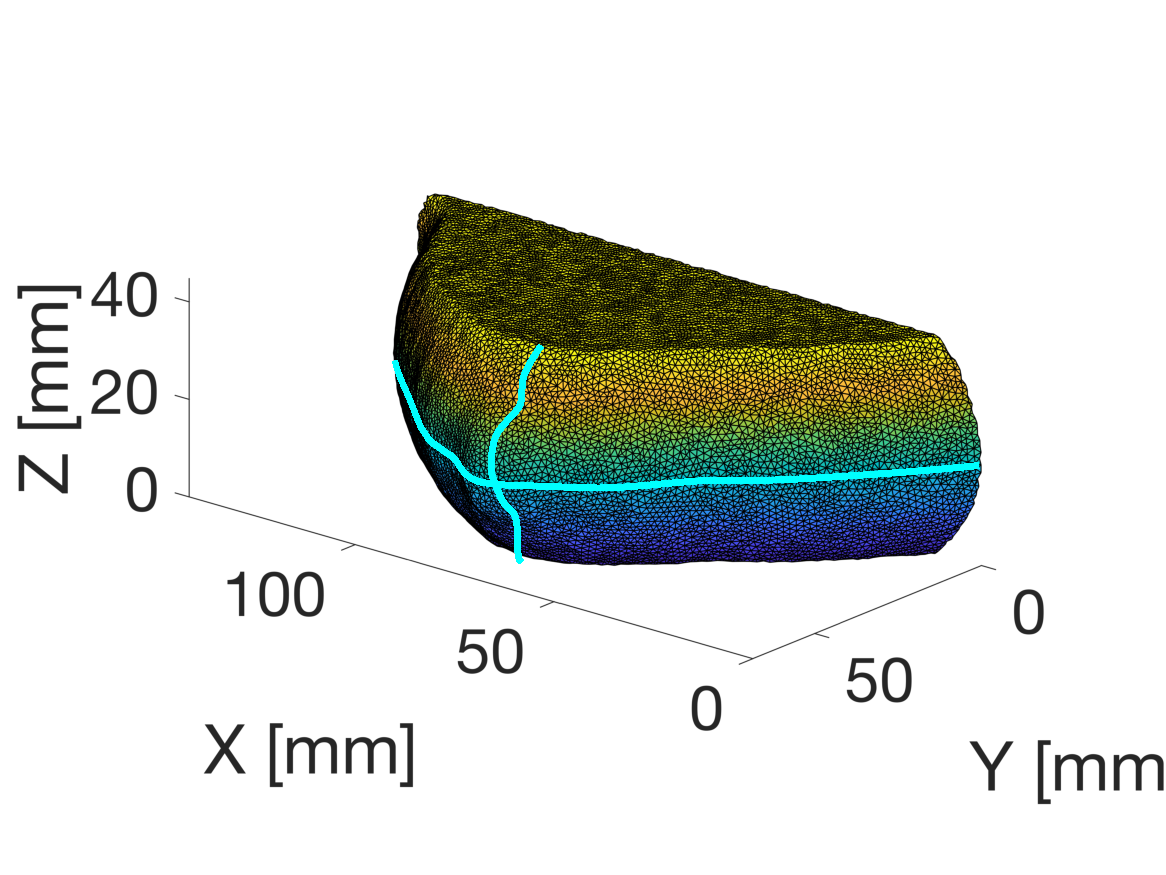
\includegraphics[width=.32\textwidth]{fig/omci/mesh_dbt.pdf}}
	\subfigure[]{\label{fig:mesh_extrude}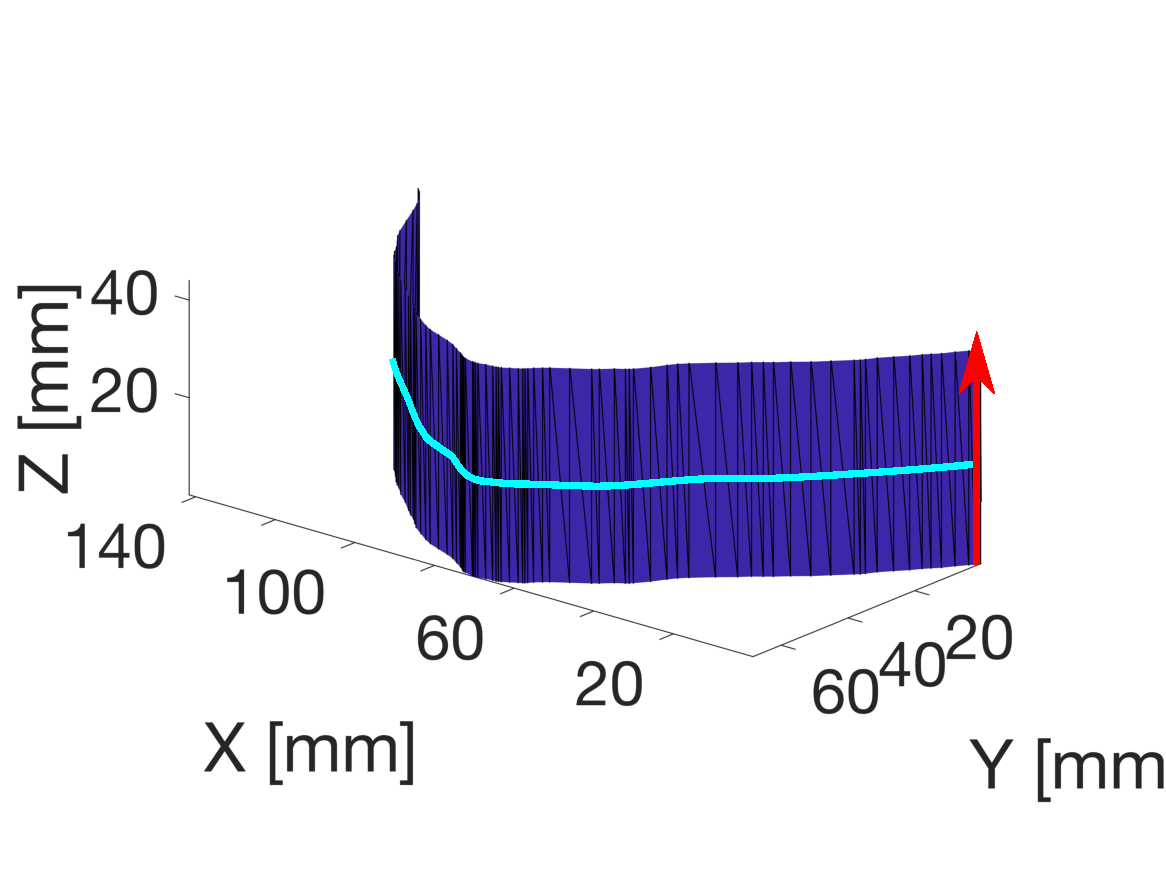
\includegraphics[width=.32\textwidth]{fig/omci/surf_ext.pdf}}
	\subfigure[]{\label{fig:mesh_topsweep}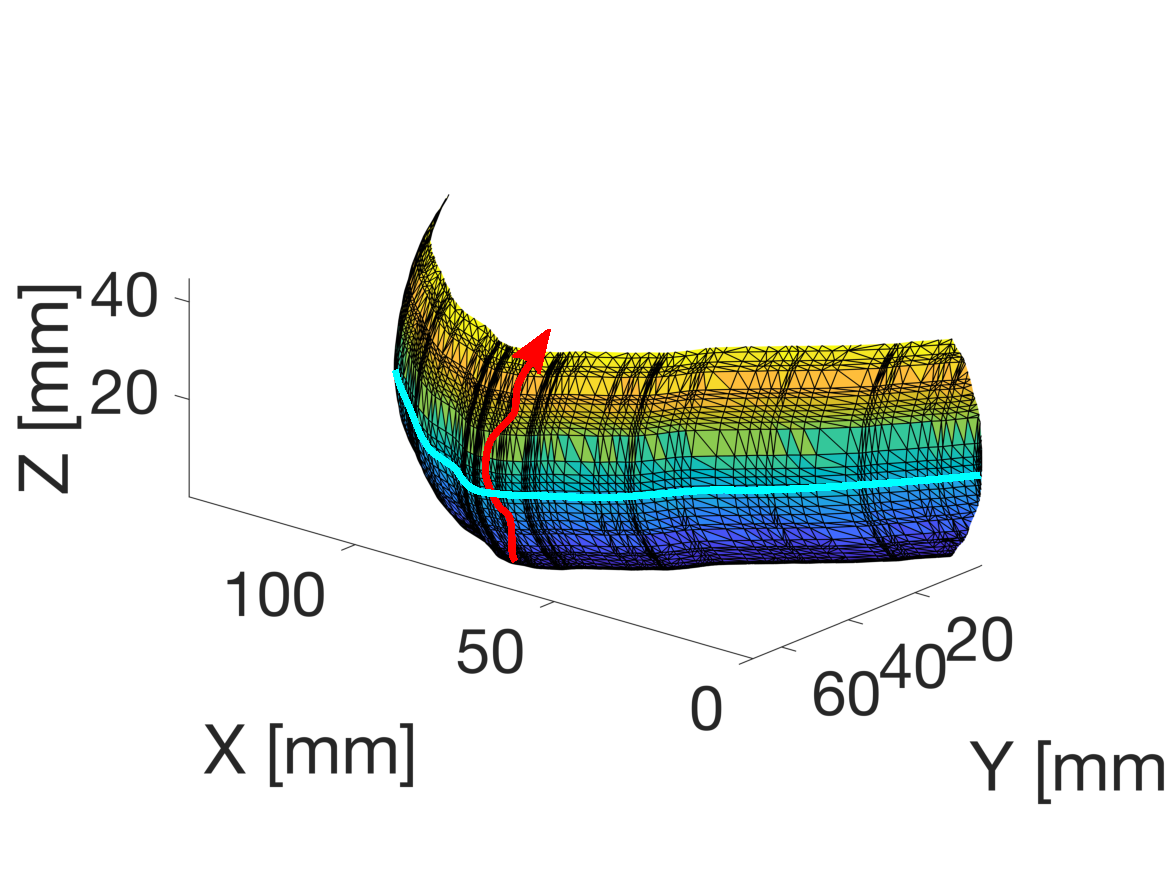
\includegraphics[width=.32\textwidth]{fig/omci/surf_top.pdf}}
	\subfigure[]{\label{fig:mesh_sidesweep}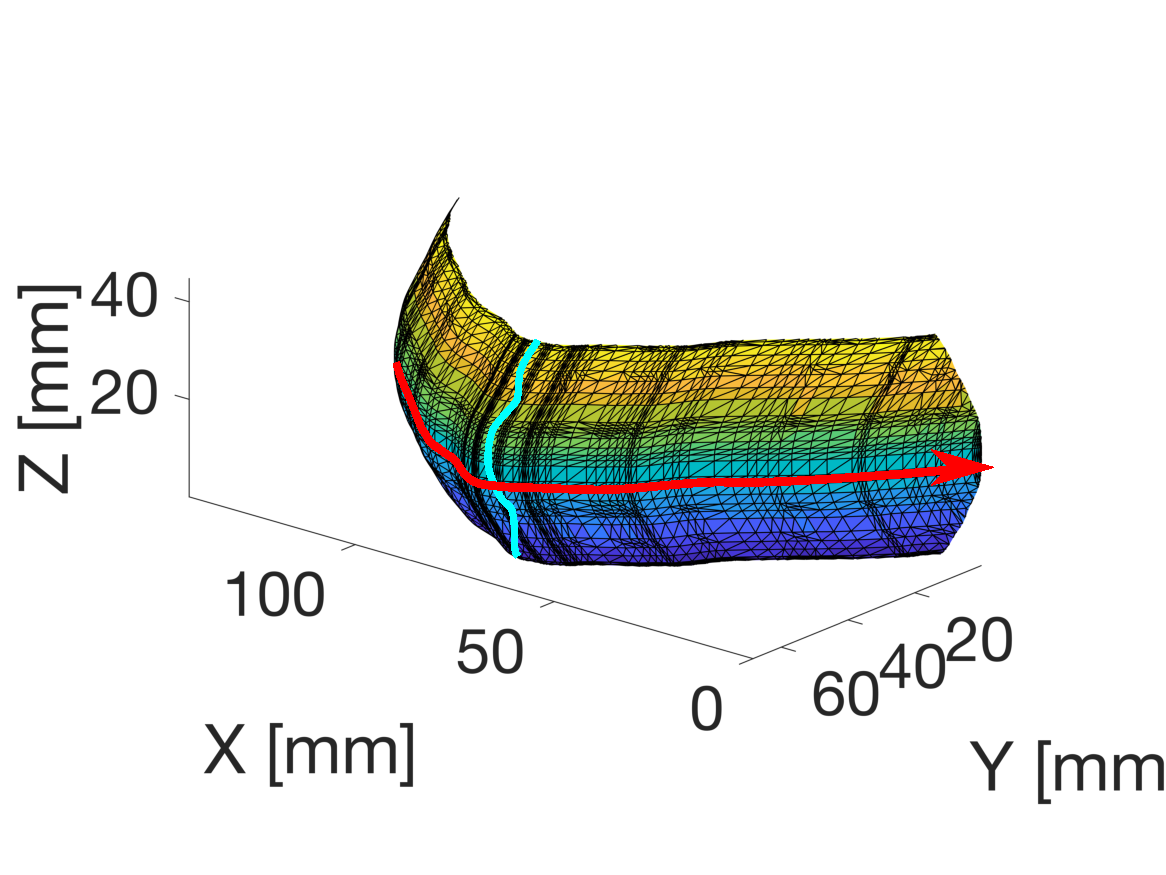
\includegraphics[width=.32\textwidth]{fig/omci/surf_side.pdf}}
	\subfigure[]{\label{fig:pcmergea}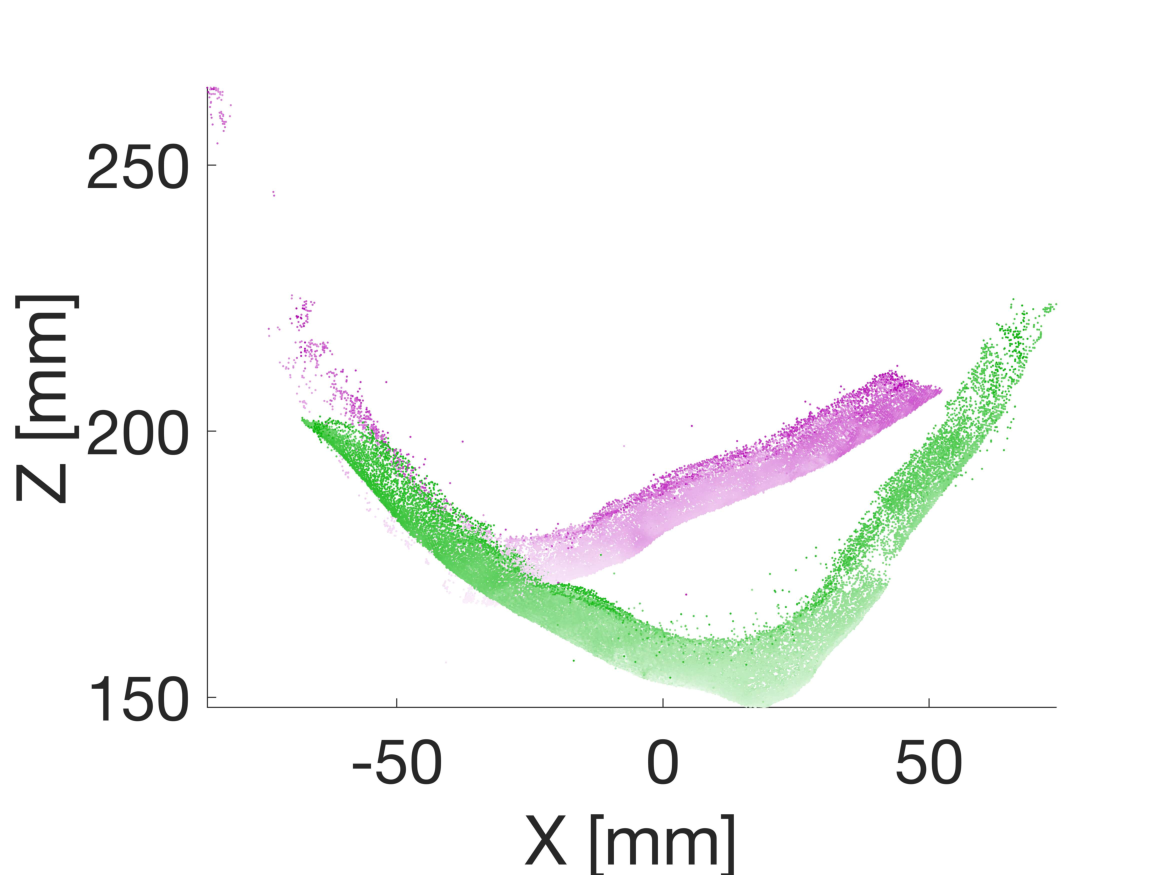
\includegraphics[width=0.32\textwidth]{fig/omci/PC_dual.pdf}}
	\subfigure[]{\label{fig:pcmergeb}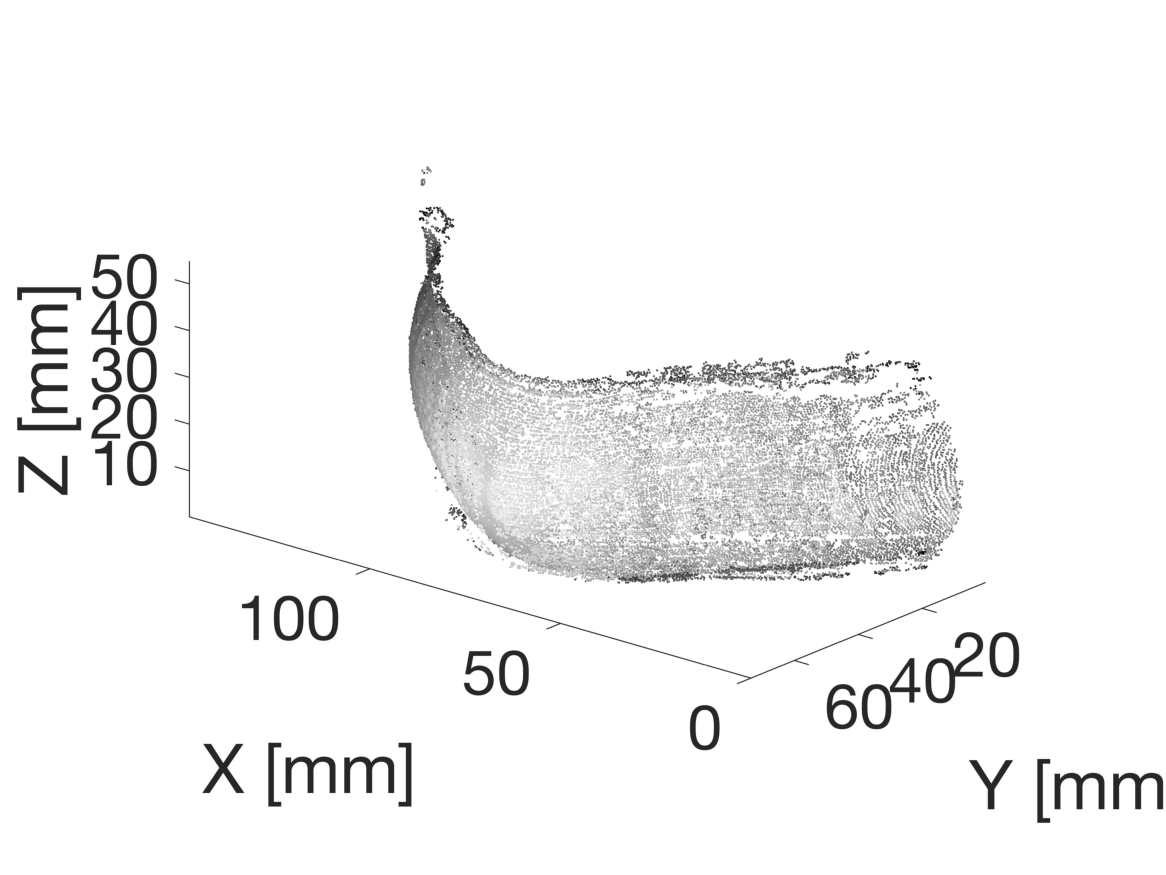
\includegraphics[width=0.32\textwidth]{fig/omci/PC_merged.pdf}}
	\end{center}
	\caption{(a) Surface mesh of a digital breast tomosynthesis model obtained from The Cancer Imaging Archive~\cite{Clark2013}. Blue cyan lines show the $x/y$ and $y/z$ breast contours from the top and side views. (b) Estimate of the \ac{DBT} surface using the extrusion method in which the contour (cyan) is extruded to the thickness of the breast along the $z$ axis. (c) The top-sweep method uses the $x/y$ contour as the profile (cyan) and the $y/z$ contour as the path to sweep (red). (d) The side-sweep method uses the $y/z$ contour as the profile (cyan) and the $x/y$ contour as the path to sweep (red). (e) point-clouds from both camera-projector pairs were generated by scanning a 3-D printed model of the \ac{DBT} breast using the \ac{SLI} system. The green (Camera 1) and magenta (Camera 2) point-clouds are in the respective camera coordinates. (f) Merged and denoised point-cloud in the projector's coordinates.} 
	\label{fig:meshes}
\end{figure} 

\subsubsection{Structured light imaging surface mesh generation}
The \ac{SLI} system estimates the surface of the compressed breast from the captured images while the breast is illuminated with Gray-code sequence patterns. Each camera-projector pair's extrinsic parameters are used to generate a point-cloud in each camera's reference frame using Scan3d-Capture~\cite{Moreno2012a} [Fig.~\ref{fig:pcmergea}]. The alignment of each camera-projector pair point-cloud is done by a rigid transformation of each point-cloud to the projector's coordinates. The point-clouds are then down-sampled using a box grid filter and merged to a single point with normal properties averaged~\cite{Pomerleau2013}. Denoising is then performed to remove outliers~\cite{Rusu2008}. The point-cloud is trimmed in the $z$ direction to the height of the \ac{DBT} breast measured by the linear encoder [Fig.~\ref{fig:pcmergeb}]. The trimmed point-cloud is first converted to a mesh using a crust algorithm~\cite{Crust1999} prior to being cropped by a bounding-box mesh with height matching the breast thickness to form a closed surface mesh. 

\subsubsection{Surface estimation error}
The surface estimation error, $E_s$, of each surface estimation method is computed by comparing the nodes in each surface mesh to the nodes in the \ac{DBT} mesh. The residual for each node in the surface mesh is the shortest distance from that node to the \ac{DBT} mesh. The \ac{SLI} output mesh is linearly translated (rotation and translation only) into the projector's frame using the projector's extrinsic parameters prior to determining residuals. $E_s$ is defined as the average residual of all nodes for a particular surface estimation method. 

%%% Subsection %%%
\subsection{Evaluation of the impact of surface errors on DOT image reconstructions}
Simulations were conducted to evaluate the impact of surface estimation accuracy on \ac{DOT} reconstruction accuracy for inclusions of various depths. Breast surface meshes were converted to volumetric meshes with optical inclusions and the mean squared error of wide-field \ac{DOT} reconstructions was calculated for each estimation method. 

\subsubsection{Assessment of reconstruction accuracy}
The effect of different surface estimations on lesion reconstruction was quantified using simulations of \ac{CW} pattern-illumination sources. A 5~mm radius spherical inclusion was added at the mid-plane of each volumetric mesh at distances of 5 to 45~mm away from the nipple. The $x$ and $z$ coordinates of the inclusion were fixed at 68 and 22~mm, respectively. The forward simulation was conducted on a ground truth volumetric mesh consisting of the \ac{DBT} volumetric mesh and a spherical inclusion. The non-linear image reconstruction of tissue properties was calculated using an iterative Gauss-Newton method in which a series of corrective terms were added to an initial guess. The reconstruction resulted in distributions, $\mathrm{\mu_{a}}_{i}$, representing the resulting 3-D absorption coefficient ($\mu_a$) maps at the $i^{th}$ node for each simulated tumor location and surface model.

\subsubsection{Reconstruction error assessment}
We use \ac{MSE} to determine the accuracy of the image reconstruction resulting from each breast mesh. To compute the \ac{MSE}, we first interpolate the reconstructed absorption map, $\mu_a$, to the \ac{DBT} mesh, and then subtract the interpolated $\mu_a$ at each node $i$, with the corresponding ground truth absorption value defined on the same node, expressed as
\begin{equation}
\label{eq:mse}
\mathrm{MSE} = \frac{1}{N}\sum_{i=1}^{N}(\mathrm{\mu_{a}}_{i} - \mathrm{\mu_{a0}}_i)^{2},
\end{equation}
where $N$ is the total node number; $\mathrm{\mu_{a}}_i$ and $\mathrm{\mu_{a0}}_i$ define the recovered and ground truth $\mu_{a}$ values, respectively, at the $i^{th}$ node in the \ac{DBT} mesh.



\section{Results}
\label{chap:omci:results} 
Results from the characterization of the \ac{SLI} subsystem are broken down into three parts. We will first report the projector and camera re-projection errors of our \ac{SLI} calibration using the calibration checkerboard. We then quantify the error of surface estimation methods in estimating the surface shape of the \ac{DBT} breast. Finally, we show the effect of different surface estimation methods on optical property reconstruction using simulations of continuous wave pattern-illumination sources. 


%%% Subsection %%%
\subsection{Camera-projector calibration and surface acquisition}
\label{ssec:calibrationresults}
Our dual-camera \ac{SLI} system was calibrated in a dark room using a checkerboard with 5$\times$7 internal corners with 1$\times$1~cm$^2$ black and white squares. The calibration checkerboard was printed and adhered to a black Delrin surface to ensure it remained planar. To account for varying breast shapes and curvatures, the checkerboard was placed at 7 locations. At each location, camera images were captured for 5 board orientations: 1) normal to the $y$-axis [see Fig.~\ref{fig:mammography_top}], 2) rotated left and 3) rotated right by 30 degrees relative to the $x$-axis, and 4) tilted forward and 5) tilted backward by 30 degrees in the $y/z$ plane [Fig.~\ref{fig:mammography_side}]. This results in a total of $7\times5=35$ checkerboard positions within the camera and projector field-of-views (Fig.~\ref{fig:mammographysetup}). Each rotation and tilt was measured manually using a printed protractor. The projector's resolution is 1280$\times$720 pixels and the resolution of the cameras is 1600$\times$896 pixels. Using a Gray-code of bit-length $P=9$, we acquire $P\times 4 + 2 = 38$ images (see Section~\ref{sec:sli}) at each board orientation/position placement. An exposure time of 0.25 seconds per image per camera results in a total one-time calibration time of $38 \times 7 \times 5 \times 2 \times 0.25 = 665$ seconds. The first camera-projector pair (Camera 1 with projector) resulted in a camera and projector re-projection error of 0.4089 and 0.2282 pixels, respectively. The second camera-projector pair resulted in a camera re-projection error of 0.4368 pixels and a projector re-projection error of 0.2889 pixels.

A re-calibration is only necessary when the relative position of the cameras and projector is changed. Once calibrated, the \ac{SLI} system can acquire a surface scan in about 35 seconds, including 16 seconds for adaptively adjusting the intensity scaling factor $\alpha$ for both cameras (see Section~\ref{sec:special} for details) and 19 seconds for image acquisition ($38 \times 2\times 0.25 = 19$ s).

%%% Subsection %%%
\subsection{Surface estimation errors}
\begin{table}
    \centering
    \caption{Mean and standard deviation of the residuals of each point in a surface estimation mesh compared to the original \ac{DBT} breast mesh.}
    %\resizebox{\textwidth}{!}{%
        \begin{tabular}{lcccc}
        \toprule
         & Extrusion & Top-Sweep & Side-Sweep & \ac{SLI} \\ \midrule
        Surface estimation error, $E_s$ [mm] & 6.8353 & 0.3772 & 0.4726 & \multicolumn{1}{l}{0.2543} \\
        Standard deviation [mm] & 2.8671 & 0.3029 & 0.3370 & 0.2723 \\ \bottomrule
        \end{tabular}%
    %}
    \label{tab:residuals}
\end{table}

The \ac{DBT} breast model was 3-D printed (Ender 5, Creality, China) with a 0.1~mm layer height using white \ac{PLA} filament. The 3-D printed \ac{DBT} breast was placed in between the compression plates, compressed to the thickness of the printed \ac{DBT} phantom, and scanned using the dual-camera \ac{SLI} system. The saturation scaling factors $\alpha$ were automatically determined using twenty iterations, resulting in a $\alpha=0.8$ for both cameras. The two point-clouds from each camera-projector pair were transformed to the projector's coordinates, down-sampled, and merged prior to being denoised with the number of nearest neighbor points set to four and the outlier threshold set to one standard deviation from the mean of the average distance to those four neighboring points. The resulting point-cloud from the \ac{SLI} system scan has 35,256 points.

Table~\ref{tab:residuals} shows the mean and standard deviation of the residual of all the nodes in the estimated breast surface mesh. The $z$-extrusion method (EXT) results in the largest error ($E_s$) of all compared methods. While the top-sweep, side-sweep, and \ac{SLI} methods all had similar standard deviations, the \ac{SLI} method resulted in the smallest $E_s$.

%%% Subsection %%%
\subsection{Mean square error of optical property reconstruction}
\begin{figure}
	\begin{center}
	    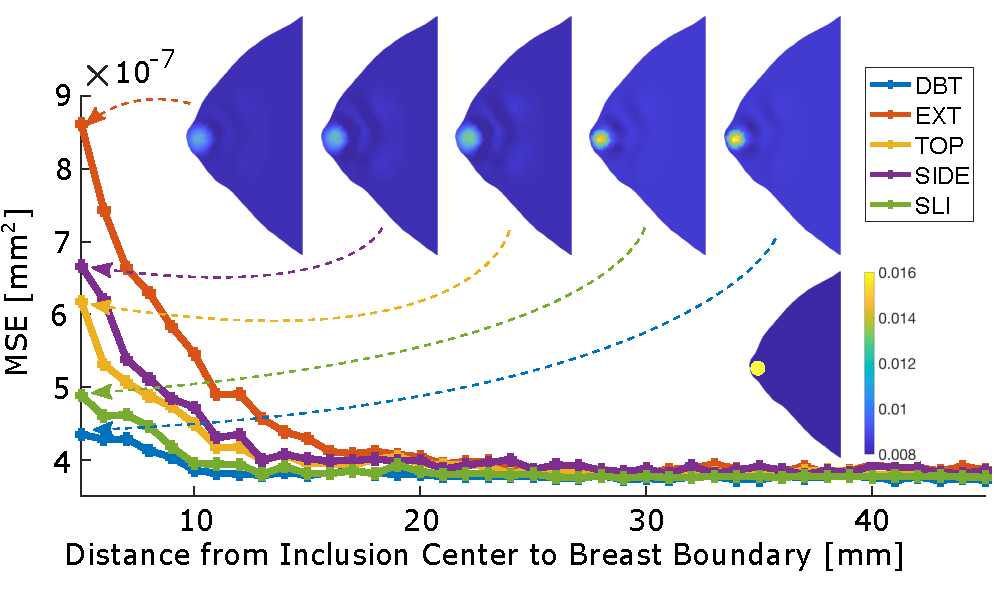
\includegraphics[width=.9\textwidth]{fig/omci/mse.pdf}
	\end{center}
	\caption{A comparison between the mean squared error (\ac{MSE}) of the reconstructed absorption map using 4 estimated surfaces (EXT - $z$-axis extrusion, TOP - sweeping $x/y$ contour along $y/z$ contour, SIDE -- sweeping $y/z$ contour along $x/y$ contour, and \ac{SLI} -- surface acquired from our \ac{SLI} system) as well as the ground truth surface (\ac{DBT}). A 1~cm diameter spherical inclusion is moved away from the breast surface at various depths between 5 and 45~mm in 1 mm increments. Image slices (in $x/y$ plane) of the reconstructed absorption coefficient ($\mu_a$ in mm$^{-1}$) (top-row) and the ground truth $\mu_a$ (bottom-right) are shown as insets.}
	\label{fig:mse}
\end{figure} 

\ac{DOT} reconstructions were performed using our in-house data analysis toolbox, Redbird-m~\cite{Redbird2008}. An $L$-curve analysis is used to determine the regularization parameter as $3.16\times 10^{-10}$, which is fixed over 10 Gauss-Newton iterations. The absorption coefficient of the spherical inclusion was set to be twice ($\mu_a=0.016$/mm) that of the background tissue ($\mu_a=0.008$/mm). The reduced scattering coefficient $\mu_s'$ was set to $1$~mm$^{-1}$ for both breast and inclusion tissues. A set of 32 (16 vertical, 16 horizontal) moving-bar source patterns~\cite{Yao2015} covering an area of 40$\times$40~mm$^2$ was centered at the spherical inclusion. Iso2Mesh was used to interpolate nodal values from the reconstructed mesh to the ground truth mesh based on linear interpolation in order for all reconstructed meshes to have the same number of nodes.

The \ac{MSE} errors from these reconstructed images are summarized in Fig.~\ref{fig:mse}, showing the effect of different surface estimation methods on the accuracy of optical property recovery. Overall, surface mesh accuracy appears to have a notable impact on relatively shallow tumors, with a depth of less than 25~mm. \ac{MSE} values obtained using the \ac{SLI} method closely follow those using the ground truth \ac{DBT} mesh for most inclusion depths. The top- and side-sweep-based meshes followed similar trends, however, reporting higher errors compared to \ac{SLI} especially when the tumor is relatively shallow. The maximum \ac{MSE} value for the \ac{SLI} mesh at a distance of 5~mm from the surface ($4.89\times 10^{-7}$~mm$^2$) was 23\% higher than the maximum \ac{MSE} value for the \ac{DBT} mesh ($4.35\times 10^{-7}$~mm$^2$). In contrast, the single-axis-extrusion method (EXT) \ac{MSE} was nearly twice higher ($8.62\times 10^{-7}$ mm$^2$) than that from the \ac{DBT} mesh. Although the \ac{DBT} and \ac{SLI} mesh \ac{MSE}s plateau to their minimum around 15~mm from the surface, top-, side-, and extrusion-based mesh \ac{MSE}s continue to decrease until a depth of 25~mm. Beyond the depth of 25 mm, the errors between different methods become minimal.

\subsection{Full system \textit{in-vivo} patient results}
\begin{figure}
    \begin{center}
    \subfigure[]{\label{fig:PatientResultsA}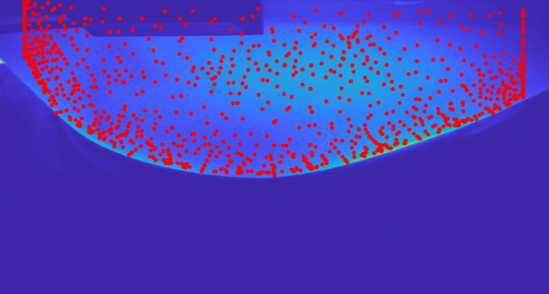
\includegraphics[width=.4\textwidth]{fig/omci/SLIMeshC.png}}
    \subfigure[]{\label{fig:PatientResultsB}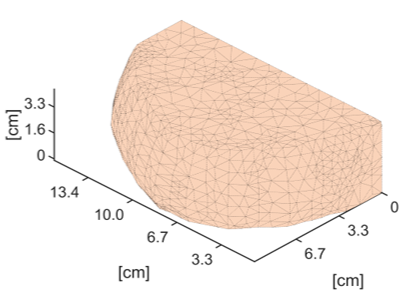
\includegraphics[width=.4\textwidth]{fig/omci/SLIMeshD.png}}
    \subfigure[]{\label{fig:PatientResultsC}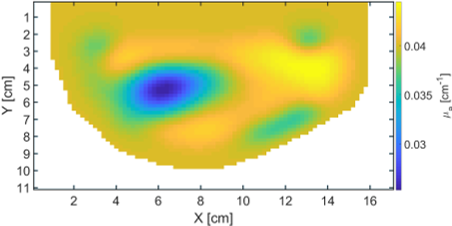
\includegraphics[width=.4\textwidth]{fig/omci/PatientResultsA.png}}
    \subfigure[]{\label{fig:PatientResultsD}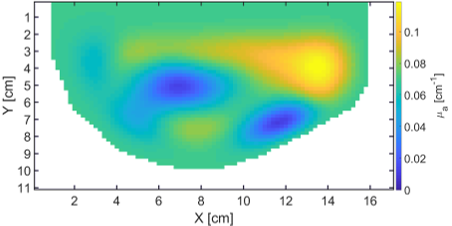
\includegraphics[width=.4\textwidth]{fig/omci/PatientResultsB.png}}
    \end{center}
    \caption{\textcolor{red}{These images will be replaced with patient data showing SLI in a healthy volunteer. I will also show reconstructed results and will cite Edward + Miguel. Edward to provide me with patient IDs that have good SLI acquisitions. } (b) The generated 3D breast-shaped mesh from a \ac{SLI} measurement on a healthy patient.} 
    \label{fig:PatientResults}
\end{figure} 

%Danvers, IRB approved, healthy subject, prior x-ray within X months.
%Acquisition time, time in compression for each breast. 
%Make sure patient we choose has a nipple (so we can see the \ac{SLI} recovery). 
%Find a patient with registered data. 



\section{Discussion}
\label{chap:omci:discussion}

% SLI results - reprojection errors
The camera and projector re-projection errors in Section~\ref{ssec:calibrationresults} represent an average error of fewer than 0.5 pixels in estimating the corner locations of a calibration checkerboard placed between 50 and 250~mm away [Fig.~\ref{fig:mammography_side}] from the projector for all 35 checkerboard positions. Although the same illumination patterns and calibration checkerboard positions were used to calibrate each camera-projector pair, we find a slightly better calibration accuracy when the projector is paired with Camera 1 since Camera 1 is closer to the projector's lens (Fig.~\ref{fig:mammographysetup}). The discrepancy in the re-projection errors of the two pairs is due in part to the asymmetry of the dual-camera setup. The asymmetry arises from the projector offset relative to its housing, making one camera closer to the projector than the other [Fig.~\ref{fig:mammography_top}]. 

% SLI results - surface errors
From Table~\ref{tab:residuals}, the single-axis extrusion method resulted in the highest surface error because it does not account for the curvature of the breast in the $y/z$ plane [Fig.~\ref{fig:mesh_extrude}]. Table~\ref{tab:residuals} indicates that, on average, points in the extrusion-method-derived surface estimation mesh are approximately 6.84~mm away from the \ac{DBT} mesh. The top- and side-sweep methods decrease the surface estimation error by incorporating a second breast contour from the $y/z$ plane [Figs.~\ref{fig:mesh_topsweep} and \ref{fig:mesh_sidesweep}]. Both methods improve the accuracy of surface estimations by approximating the 3-D curvature of the breast. We want to point out that both top-sweep and side-sweep methods require an additional camera to obtain two orthogonal views of the breast~\cite{Pinto2020}, which does not necessarily lead to simplified hardware compared to the \ac{SLI} setup considering the mounting space constraints and lighting conditions~\cite{Rodriguez2017}. While also requiring two cameras, our mammography-tailored \ac{SLI} system can produce sub-millimeter resolution of the surface compared to the reference \ac{DBT} breast model based on Table~\ref{tab:residuals}.

% SLI results - MSE
Our results also demonstrated that the improvement in surface estimation accuracy can lead to improved \ac{DOT} reconstruction accuracy. Fig.~\ref{fig:mse} shows using breast surfaces derived from \ac{SLI} can accurately recover the absorption profile compared to those recovered using the ground-truth (\ac{DBT}) mesh at most tested tumor depths. For superficial/shallow ($<$ 10~mm) tumors, the top- and side-sweep surface estimation methods followed similar trends to each other, reporting \ac{MSE}s about 50\% higher compared to those from using ground-truth (\ac{DBT}) surface models, and about 30\% higher than those from using \ac{SLI} surfaces. As expected, the effect of the surface accuracy decreases as the inclusion is moving further away ($>$ 25~mm) from the skin.

% Patient results - to be added after patient results are added
%In patient measurements, the \ac{SLI} subsystem successfully adjusted its projector intensity to prevent webcam saturation. The recovered bulk breast tissue optical properties from the \ac{FD} subsystem followed the reported values from our group~\cite{Fang2009} and others~\cite{Durduran2002}. Moreover, the 3-D reconstruction of the tissue physiology parameters resembles the internal breast tissue structures (i.e. adipose, muscle, and fibroglandular tissue) described previously~\cite{Fang2009}, denoting the capability of our system to resolve breast compounds.

%limitations
Despite the ability to produce sub-millimeter resolution of breast surfaces in poorly lit and confined mammography-like settings, both our \ac{SLI} system and our analysis have limitations. Firstly, the span of the output point-cloud from our \ac{SLI} system is limited to the area of the breast that is well-illuminated by the projector. As a result, tissue boundaries near the chest wall or those in direct contact with the compression plate may not be well covered due to the limited angles of the projector/camera line-of-sight. Still, for \ac{DOT} of a compressed breast, capturing a significant portion of the front-facing breast tissue as our system does, provides quantitative differences in reconstructions, as shown above. Future improvement of this system should consider using more compact, wide-angle projectors, higher resolution cameras, and patterns with higher order binary codes to both expand the field-of-view and increase the point-cloud resolution. Secondly, a 3-D printed breast model was used to experimentally compare different shape acquisition methods. Different choices of extruder sizes, filament colors, and printing techniques could impact the surface texture of the printed phantom and slightly alter the surface estimation errors. Finally, the quantification of reconstruction errors was based on simulations using a single set of pre-determined breast models, tumor size and shape, tumor contrast, and wide-field pattern size. An experimental validation using heterogeneous phantoms may produce more realistic comparisons.

% CONCLUSION GOES INTO THE CONLUSION OF THE ENTIRE THESIS

% --- EOF ---